\section{Capteurs externes}

Ces capteurs fournissent un signal qui sera corrélé avec la respiration. Ils vont permettre par la suite de faire correspondre les données acquises avec une phase particulière du mouvement respiratoire.

\subsection{Spiromètre}

Le spiromètre est un capteur externe placé sur la bouche du patient et qui permet de mesurer les déplacements d'air dans le système respiratoire~\cite{guivarc2004synchronization}. Les spiromètres mesurent un débit ou un volume d'air inspiré/expiré (voir illustration figure \ref{fig:spirometre}). A partir de l'une des grandeur, il est possible d'estimer l'autre facilement. L'avantage du spiromètre est qu'il permet d'accéder à une mesure caractérisant directement la respiration du patient, et n'est pas sujet à des perturbations externes (mouvements involontaires par exemple). Par contre cela demande un appareillage qui peut être assez invasif pour le patient.

\begin{figure}[h!]
	\begin{center}
		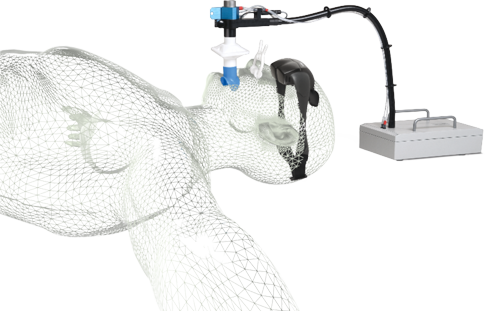
\includegraphics[width=12cm]{images/spiro}
	\end{center}
	\caption{spiromètre Syn'r : on peut voir le système de mesure de la respiration ainsi qu'un système de moniteurs implantés dans les lunettes pour aider le patient à contrôler sa respiration} 
	\label{fig:spirometre}
\end{figure}

\subsection{Ceinture}

Pour mesurer le signal respiratoire, il est possible d'utiliser un capteur qui va mesurer le périmètre du thorax. L'extension de cette ceinture va correspondre aux mouvements de la cage thoracique et de l'abdomen pendant la respiration du patient. C'est une mesure indirecte de l'amplitude du mouvement respiratoire utilisée couramment en routine clinique \todo{donner ref de raison utilisation}. 

Différentes technologies existent pour mesurer cette informations (RespiTrace R250 de Studley. Data Systems, Respiratory Belt Transducer de ADInstruments, ...). Elles sont basées sur plusieurs effets (résisitif, inductif...) et ont l'avantage d'avoir un faible coût et de ne pas perturber le patient.

\subsection{Basés caméras}

Des caméras peuvent être utilisées pour estimer le mouvement respiratoire. Une des techniques consiste à utiliser des informations surfaciques en reconstruisant en 3D certaines parties du corps à l'aide de plusieurs caméras (avec ou sans marqueurs) ou de caméra temps de vol. Cela permet d'avoir plus d'informations sur la respiration.

Une autre technique consiste à installer un marqueur sur le corps du patient et de relever les déplacements de ce marqueur à l'aide d'une caméra. Un tel système est décris dans~\cite{nehmeh2002effect} : Respiratory Gating System de Varian Medical Systems (voir figure \ref{fig:RGSdeVarian}).

\begin{figure}[h!]
	\begin{center}
		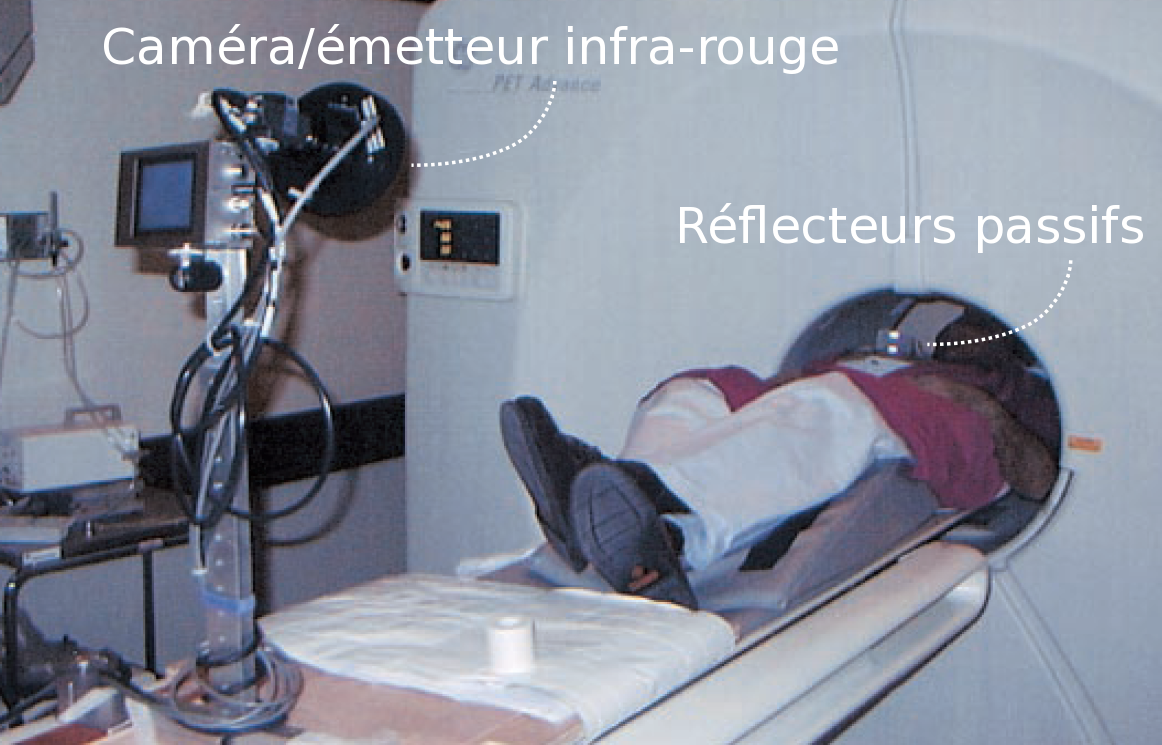
\includegraphics[width=12cm]{images/varian}
	\end{center}
	\caption{Photographie du système RGS de Varian medical Systems en action : une caméra va détecter le déplacement d'une zone du thorax en mesurant le déplacement de marqueurs placés sur un bloc plastique. } 
	\label{fig:RGSdeVarian}
\end{figure}

Ces techniques ont l'avantage d'être moins invasives et plus facilement acceptées par le patient. Cependant, elles sont beaucoup plus sensibles aux mouvements parasites.

\subsection{Techniques basées sur les images TEP}

Une publication utilise des images TEP pour déduire le signal respiratoire~\cite{bundschuh2007postacquisition} : les images TEP sont reconstruites par pas temporel de 0.5s. La position axiale du barycentre de chaque image donne une estimation du signal respiratoire. Cette technique donne les meilleurs résultats pour une zone d'interêt centrée sur une tumeur de forte intensité.

\section{Estimation du champ de mouvement}

Le signal respiratoire acquis par les méthodes précédemment cités est utilisé pour décomposer les données acquises en TDM ou TEP en plusieurs phases, chacune correspondant à un instant du cycle. Ces informations sont utilisées pour assembler les données acquises en \todo{traduire} ``bins'', reconstruits indépendamment. Ces reconstructions vont être utilisées pour estimer les champ de mouvements à l'aide de techniques de recalage.

\subsection{Image TDM 4D}

Les images TDM peuvent être acquises en mode dynamique de manière à obtenir un ensemble d'image couvrant tout le cycle respiratoire \cite{lamare2007list, qiao2006motion}. Les données des 

Des algorithmes de recalage sont utilisés de manière à déduire le champ de mouvement. Bien que les images soient de bonne qualité et permettent une estimation précise du champ de mouvement, cela demande une exposition supplémentaire aux rayonnements X.

Plusieurs publications basées sur des simulations se servent des cartes de labels utilisées pour la simulation pour réaliser les estimation de mouvements. Cela donne une estimation dans le ``meilleur des cas'', où l'image TDM est parfaitement en phase avec les images TEP.

\subsection{Image TEP 4D}

Les données regroupées selon l'instant du cycle auquel ils appartiennent \cite{dawood2008respiratory, dawood2006lung}. Les image sont reconstruites indépendamment  sans correction d'atténuation, puis un algorithme de recalage est utilisé pour estimer le champ de mouvement. L'avantage de cette technique est de ne pas nécessiter d'irradiation ni de temps supplémentaire. Cependant, les images reconstruites sont de mauvaises qualité et peuvent réduire la précision du champ de mouvement estimé.

\section{Modèle}

Une autre voie est en cours de développement basée sur la création d'un modèle de respiration généralisé adapté à chaque patient à partir de données réduites. Fayad \cite{fayad2010application} propose une méthode basée sur l'analyse en composantes principales pour modéliser les mouvements. Ce modèle est ensuite adapté à un patient à partir de deux images TDM prises à des instants différents du cycle. Enfin, une caméra 3D permettant d'obtenir la surface du corps du patient est utilisé pour synchroniser le mouvement respiratoire et affiner le modèle.

L'avantage de ce modèle est qu'il est totalement continu, et permet l'extraction d'un nombre arbitraire de phases.